\documentclass[conference]{IEEEtran}
\usepackage{graphicx}
\usepackage{stfloats}

\ifCLASSINFOpdf
  % \usepackage[pdftex]{graphicx}
  % declare the path(s) where your graphic files are
  % \graphicspath{{../pdf/}{../jpeg/}}
  % and their extensions so you won't have to specify these with
  % every instance of \includegraphics
  % \DeclareGraphicsExtensions{.pdf,.jpeg,.png}
\else
  % or other class option (dvipsone, dvipdf, if not using dvips). graphicx
  % will default to the driver specified in the system graphics.cfg if no
  % driver is specified.
  % \usepackage[dvips]{graphicx}
  % declare the path(s) where your graphic files are
  % \graphicspath{{../eps/}}
  % and their extensions so you won't have to specify these with
  % every instance of \includegraphics
  % \DeclareGraphicsExtensions{.eps}
\fi
% graphicx was written by David Carlisle and Sebastian Rahtz. It is
% required if you want graphics, photos, etc. graphicx.sty is already
% installed on most LaTeX systems. The latest version and documentation
% can be obtained at: 
% http://www.ctan.org/pkg/graphicx
% Another good source of documentation is "Using Imported Graphics in
% LaTeX2e" by Keith Reckdahl which can be found at:
% http://www.ctan.org/pkg/epslatex
%
% latex, and pdflatex in dvi mode, support graphics in encapsulated
% postscript (.eps) format. pdflatex in pdf mode supports graphics
% in .pdf, .jpeg, .png and .mps (metapost) formats. Users should ensure
% that all non-photo figures use a vector format (.eps, .pdf, .mps) and
% not a bitmapped formats (.jpeg, .png). The IEEE frowns on bitmapped formats
% which can result in "jaggedy"/blurry rendering of lines and letters as
% well as large increases in file sizes.
%
% You can find documentation about the pdfTeX application at:
% http://www.tug.org/applications/pdftex

% correct bad hyphenation here
\hyphenation{op-tical net-works semi-conduc-tor}


\begin{document}

\title{Cuttlefish: A Library For Building Distributed Neural Networks}

\author{\IEEEauthorblockN{Abu Kamruzzaman\IEEEauthorrefmark{1},
Rania Mohammedameen Almajalid\IEEEauthorrefmark{2}, Yu Hu\IEEEauthorrefmark{3} and
Tereas Nicole Brooks\IEEEauthorrefmark{4}}
\IEEEauthorblockA{Computer Science,
Pace University\\
Pleasantville NY\\
Email: \IEEEauthorrefmark{1}ak91252p@pace.edu,
\IEEEauthorrefmark{2}ra56319p@pace.edu,
\IEEEauthorrefmark{3}Rain0613@hotmail.com,
\IEEEauthorrefmark{4}tb93141n@pace.edu}}
\maketitle

% make the title area
\maketitle

% As a general rule, do not put math, special symbols or citations
% in the abstract
\begin{abstract}
This paper will discuss the implementation of Cuttlefish, a library for building configurable, fault tolerant, distributed neural networks. Cuttlefish is built on top of the Distributed TensorFlow library. It uses Docker containers to represent units or neurons in the a neural network. More specifically each container (neuron) will run as a service that can communicate with other neurons in the network. Our neural network will be a n layered network, implemented and configured to run on Amazon Web Service's Elastic Container Service (ECS).
\end{abstract}

\IEEEpeerreviewmaketitle



\section{Introduction}
Machine learning and more specifically the use of Neural Networks have many applications in both the research and commercial software. Though most machine learning techniques and algorithms employed today were developed over 20 years ago the rise of cheap, powerful processors (GPUs and CPUs) and higher capacity storage as allowed these techniques and algorithms to be used at scale.

In this paper we will talk about the implementation of Cuttlefish, a library for building configurable, fault tolerant, distributed neural networks. We will discuss the technologies used to implement this library which includes the use of clustered Docker containers, where each container represents a neuron in the network, Distributed TensorFlow and Amazon Web Service's Elastic Container Service (ECS).

\section{Background}
[TODO: Add intro paragraph for this section]\\

\subsubsection{Docker}
Docker is the world's leading software containerization platform. Docker is open source, designed to make it easier to create, deploy, and run distributed applications inside lightweight Linux containers. It provides a way to run applications securely isolated in a container by packaging it and all its dependencies as well as libraries. Docker containers can wrap the software into a self-contained unit with a complete file-system that contains everything needed to run: operating system, code, runtime, system tools, system libraries, and configured system resources ?. etc. By using Docker containers, we can deploy, and back up a workload regardless of environment quickly and easily more than using virtual machines.

Docker allows to change any application dynamically by adding new capabilities and scaling services which makes containers more portable and flexible to use. Docker also has a mechanism for configuring and spinning up containers that should be clustered together or that are dependencies of one another.

One of the Docker advantages is simplified maintenance which means Docker minimize the efforts and risks which associates with application dependencies. The other advantage is increasing developer productivity because it decreases the time that spent setting up 

\subsubsection{TensorFlow}
TensorFlow is essentially a framework for building Deep Learning Neural Networks. It was developed by engineers and researchers working on the Google Brain Team within Google's Machine Intelligence research organization. It is an open source software library for machine learning computation using data flow graphs. Data flow graphs describe mathematical computation with nodes and edges. Each node in the graph represents mathematical operations, while edges represent the relationships between nodes. A computation expressed using TensorFlow can be executed in one or more GPUs or CPUs in a desktop, mobile device, or server with a single API.

The initial open-source release of TensorFlow supports multiple devices (CPUs and GPUs) in a single computer which is called the single-machine or single node implementation, while the distributed version supports multiple devices (CPUs and GPUs) across a cluster of machines.

\subsubsection{Amazon EC2 Container Service (ECS)}
Amazon EC2 Container Service (ECS) is high performance container management service which supports Docker containers through Management Console or Command Line Interface. It is highly scalable and allows applications to run easily on a managed cluster of Amazon Elastic Compute Cloud (Amazon EC2) instances. Amazon ECS enables applications to be scaled without any additional complexity from a single container to thousands of containers across hundreds of instances. Amazon ECS allows launch and stop container-based applications with simple API calls. 

\section{Motivation}
The initial motivation for Cuttlefish was born from the the observation that neural networks at their core are computational graphs and more specifically directed computational graphs, where each neuron in the graph is a single computation unit. This observation coupled with the understanding that in order to train models and make inference of new data presented to these models at scale, in a production environment, requires implementing neural networks in a way that enables us to infinitely scale the execution of the these computation graphs in way that allows us to leverage all available system resources.  

Tasks for training models and performing inference in neural networks are inherently parallelizable. Hence, it should be possible to implement a library that allows users to create a fault tolerant, distributed neural network, using configurable hyperparameters to drive the dynamic creation a directed graph of neurons (a neural network).  To implement this library a means of represent each node in the network physically; as a device or machine where computation execution will take place. We also need a centralized database to store intermediate values for the weight parameters each neuron calculates during model training. Moreover, the neurons in the network would need an efficient mechanism to communicate and pass data from one neuron to another. Lastly, we would need a mechanism to automate configuring and ''spinning up'' a neural network.  Below we briefly discuss the technologies and approaches needed to implement such a library.

\begin{figure*}
  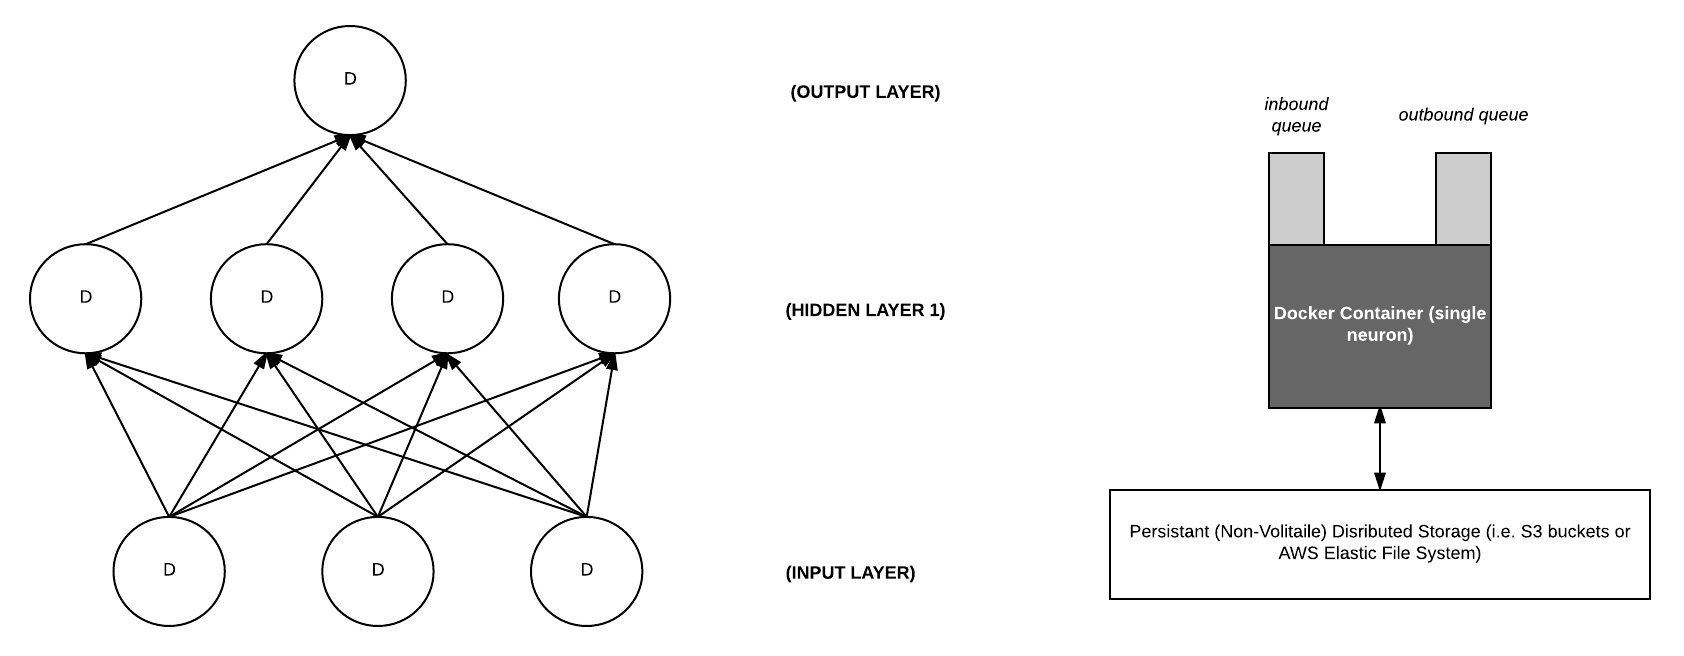
\includegraphics[width=\textwidth]{ml_figure_draft.png}
  \caption{Diagram example neural network nodes as docker containers. Note, the persistent distributed storage represent non-volatile storage for localized data per docker container. Persistent storage is needed to provide fault tolerance for shared and unshared data.}
\end{figure*}

\subsubsection{Physical Representation of Neurons: Docker Containers}
The user of Docker to represent physical a physical neuron was an natural choice because docker containers are self contained units that enable you to provide everything an application would need to run and nothing more; this includes an operating system, file system (volatile file system), and another other needed software, frameworks or tools. Using Docker's Compose tool \cite{docker-compose-doc} containers can easily be configured as dependencies of one another hence allowing you to create a cluster of containers that can be spun up together and can communicate with each other.

\subsubsection{Centralized Storage Of Weighted Model Parameters: Distributed NoSql Database}
For our centralized parameter store, because the data is not highly relational and we would need a scalable solution distributed key, value stores such a Amazon Web Services' DynamoDB would be a good fit.

\subsubsection{Interneuron Communication}
For inter-neural network communication we would need an Inbound and output queue for each neuron in the network in order to pass data such as computed weights, and training model data from node to node. To implement such communication fault tolerant message broker technologies such as rabbitmq \cite{rabbitmq-doc} or Apache Kafka \cite{kafka-doc} are good choices.

\subsubsection{Automation of ''Spinning'' Up Elastic Neural Networks}
Infrastructure orchestration software such as Kubernetes, Mesos and Amazon Web Service's Elastic Container Service are tools used in both test and production environments to automate orchestrations for creating, configuring and managing docker containers, and hence makes them a natural fit for this task.

\section{Our Approach}

** Note, this section should really be called ''Our Proposed Approach'' as is being written before we have implemented Cuttlefish and before we know more about Distributed TensorFlow's capabilities**\\

During the initial research phase of this project, we discovered Google's Distributed TensorFlow project in spirit was very similar the initial idea that motivated our research.  Distributed TensorFlow allows you to create a cluster of servers, where each worker process task is associated a server in the cluster.

Distributed TensorFlow though it is primarily used for modeling machine learning computational models is generic enough to be considered a general purpose distributed computing engine. It offers fault most of the properties we thought were paramount in implementing a library to enable building elastic distributed neural networks: fault  tolerance, a means of sharing common calculated parameters among devices in TensorFlow cluster \cite{dist-tensorflow}, cross device communication, as well as distributed execution of a computation graph among nodes in a TensorFlow cluster.  Hence, we decided to use Distributed TensorFlow as the base for the Culttlefish library.

Note that Cuttlefish defines a docker container as a single server in a TensorFlow cluster. Hence a Cuttlefish distributed neural network is simply defined as TensorFlow cluster.

\subsubsection{Computation Graph Distribution}
TensorFlow uses a greed heuristic algorithm called the ''placement algorithm'' \cite{tensor-flow-white} to determine how a computation graph will be distributed for execution among all available devices. Default supported device types are CPUs and GPUs, there is  also a registration mechanism so that users can implement and register their own device types \cite{tensor-flow-white}. TensorFlow provides an interface for users to influence how the computation graph is distributed, by allowing them to give ''hints and partial constraints'' to the algorithm \cite{tensor-flow-white}. 

Cuttlefish, will use the above described functionality along with the configuration of each docker container?s system resources (memory, number of CPUs etc) to attempt to force TensorFlow?s placement algorithm to map one node in the computation graph to one docker container.  This is will test our the viability of our motivation of using a single docker container to represent a single computational unit in a distributed neural network (neuron).

\subsubsection{Configuring Neural Network (Hyperparameters)}
With Cuttlefish users define the configuration and shape of their neural network?s hyperparameters in a yaml file. By defining these parameters as ''code'', versioning of these parameters is simple, this also allows a user to automate building these configuration files as a tasks in a larger workflow where hyperparameters are being tested for a given set of training data.

\subsubsection{Automation \& Orchestration: Creating Docker Containers As Per Cuttlefish Configuration File}
Cuttlefish?s ''build'' functionality will use the Amazon Web Services' (AWS) elastic contain service?s API \cite{ecs-api} and it's user defined elastic neural network configuration files to configure and build a distributed neural network using a cluster of docker containers (TensorFlow cluster).

With this approach, Cuttlefish takes the paradigm of infrastructure and applies it the configuring and building of a distributed neural network as a cluster of resources readily available for computation tasks.

Note, though we are using AWS' ECS \cite{ecs-doc} for orchestration for this proof of concept, tools like Kubernetes and Mesos are better choice as they offer finder grain control over configuring resource allocation per container. Fine grain control of such resources would allow for configuring and tuning system resources per neuron type, thus making the required system resources fit the computation being performed by a particular neuron. This level of control would be useful when implementing neural networks such as convolutional neural networks, where different types of neurons perform different computational tasks and hence are likely to have different resource needs.

\subsubsection{Data Set}
We are using the MINST data set for training distributed neural networks created by Cuttlefish. ?The MNIST database of handwritten digits, available from this page, has a training set of 60,000 examples, and a test set of 10,000 example.? \cite{mnist-doc} We choice the MINST data set because it is well documented, there is extensive benchmark data for it and TensorFlow as the full data set in a preprocessed ready to use format.


\section{System \& Application Architecture}
TBD

\section{Results}
TBD

\section{Improvements \& Possible Future Work}
TBD

\section{Related Work}
TBD


\section{Conclusion}
TBD


\bibliographystyle{plain}
\bibliography{ml_project_draft.bib}


\end{document}


